\documentclass[french,a4paper,11pt,oneside]{article}

\usepackage[utf8]{inputenc}
\usepackage{hyperref}
\usepackage{babel}
\usepackage{amsmath}
\usepackage{amsfonts}
\usepackage{amssymb}
\usepackage{graphicx}
\usepackage{xcolor}
\usepackage[rightlabels]{titletoc}
\usepackage{pdfpages}
\usepackage{tikz}
\usetikzlibrary{decorations.markings}
\usepackage{grffile}
\usepackage[export]{adjustbox}
\usepackage{listings}
\usepackage{datetime}  
\usepackage{sectsty}
\usepackage{python}
\usepackage{float}
\usepackage{listings}

\renewcommand{\contentsname}{Sommaire}
\renewcommand{\thesection}{\Roman{section} } 
\renewcommand{\thesubsubsection}{ } 
\definecolor{googlegreen} {HTML}{0F9D58}
\definecolor{googleblue}  {HTML}{4285F4}
\definecolor{googlered}   {HTML}{DB4437}
\definecolor{googleyellow}{HTML}{F4B400}

\sectionfont{\color{googlered} \normalfont} % sets colour of sections
\subsectionfont{\color{googlegreen} \normalfont}  % sets colour of sections
\subsubsectionfont{\color{googleblue} \normalfont}  % sets colour of sections

\begin{document}
	 \begin{titlepage}
		\centering 
		
		\vspace{1.5cm}
		
		{\huge\bfseries Fiche de lecture \par}
		\vspace{0.5cm}
		\vfill
		
		{\Large\itshape Les réseaux de neurones convolutifs dans le monde des cylindrées\par}
		\vfill
		

		{\large Auteur  \par
			GHOUIBI Ghassen \textsc{}\par}
		\vspace{1cm}
		{\large Encadrée \par
			Mr.Jean Jacques Mariage \textsc{}\par
		}
	\end{titlepage}

	\tableofcontents
	\newpage
	\section{Introduction}{
		Le mixage entre l'informatique et la mécanique se fait en toute douceur si on prend comme exemple les voitures.\\
		Dans certaines tâches les humaines sont plus rapides puisqu'ils ont acquis un point de vue humain qu'une machine n'a pas. C'est pour çelà par exemple qu'on vous demande de prouvez votre humanité à traves un formulaire facile, CAPTCHA ou autre où le but est par exemple der trouve les images qui contiennent des voitures.\\
		Pour les ordinateurs c'est un peu plus compliqué d'identifier dans des images qui contiennent des panneaux par exemple vu qu'il doivent absorber une quantité de données importantes et se dôter de performance de calcul.\\
		Les entreprises spécialisées comme \texttt{GAFA} et \texttt{Tesla} investissent des millions de dollar dans le domaine du Big Data qui est en explosition continu. Dans notre rapport on va se focaliser sur les voitures autonomes.\\
		En effet, la reconnaisance de millions d'images ou de vidéos pour identifier un contenu précis est coûteux et demande une démarche particulière et pourtant il existe très peu de techniques pour analyser ces données de manière automatisée et efficace.\\
		\subsection{Problématique}{
			Les solutions de classification d'image présentent actuellement dans les voitures intelligentes vont-elles permettre de réduire les accidents de la route ?
		}
		 \subsection{Contexte}{
			Dans ce rapport on peut définir notre contexte comme un problème de classification, d'où on va présenter quelque variante des réseaux de neurones convolutifs qui est une approche trés populaire pour résoudre des problèmes de reconnaissance de formes. 
	 	 
 	    }
	}
	
	\section{Réseaux de neurones convolutifs }{
		Les réseaux de neurones convolutifs sont des méthodes d'apprentissage supervisé, ils suivent ce cycle ci-dessous:\\
		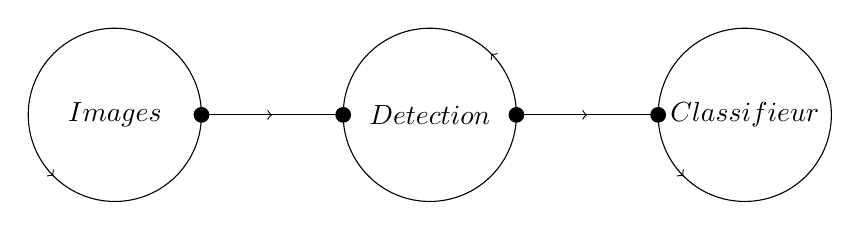
\begin{tikzpicture}
		% draw the two circles and decorate them with arrows
		\draw[
		decoration={markings, mark=at position 0.625 with {\arrow{>}}},
		postaction={decorate}
		]
		(0,0) circle (1.1) node {$Images$};
		\draw[ 
		decoration={markings, mark=at position 0.125 with {\arrow{>}}},
		postaction={decorate}
		]
		(4,0) circle (1.1) node {$Detection$};
		
		\draw[ 
		decoration={markings, mark=at position 0.625 with {\arrow{>}}},
		postaction={decorate}
		]
		(8,0) circle (1.1) node{$Classifieur$};
		
		% draw the connecting line
		\draw[ 
		decoration={markings, mark=at position 0.5 with {\arrow{>}}},
		postaction={decorate}
		]
		(1.1,0) -- (2.9,0);
		
		\draw[ 
		decoration={markings, mark=at position 0.5 with {\arrow{>}}},
		postaction={decorate}
		]
		(5.1,0) -- (6.9,0);
		
		
		
		% draw the two black dots
		\fill (1.1,0) circle (0.1); 
		\fill (2.9,0) circle (0.1); 
		\fill (5.1,0) circle (0.1); 
		\fill (6.9,0) circle (0.1); 
		\end{tikzpicture}
		\newpage
		Plus en détails la réception des images en entrées ensuite les réseaux de neurones convolutifs détectent les features de chaque image puis entraînent un classifieur dessus.\\
		
		Comme détaillé auparavant on s'intéresse au problème de classification, Le réseau va donc calculer à partir de nos entrées un score pour chaque classe, Finalement la classe sera affectée à l'objet d'entrée qui à le meilleur score.\\
		
		Une architecture de réseau de neurones se composent à traves un empilement de couches de traitement :
		\begin{enumerate}
			\item couche de convolution qui traite les données d'un champ récepteur.
			\item couche de pooling qui permet de compresser l'information.
			\item couche de correction en référence à la fonction d'activation.
			\item couche entièrement connectée qui est une couche de type perceptron.
			\item couche de perte (LOSS). 
		\end{enumerate}

		\subsubsection{Couche de convolution}{
			La couche convolution est un bloc de construction indispensable d'un CNN.\\
			Elle contient trois paramètres qui sont :\\
			\begin{itemize}
				\item La Profondeur
				\item Le Pas
				\item La marge
			\end{itemize}
			L'entrée d'une couche convolution est soit une image soit la sortie d'une autre couche de convolution. Pour calculer le nombre de neurones de sortie voici la formule: \\
			\begin{equation}\label{key}
			\underset{0}{W}=\frac{\underset{i}{W}- K + 2P}{S} +1
			\end{equation}
			\begin{itemize}
				\item \texttt{Wi} volume d'entrée
				\item \texttt{K} nombre de champs récepteurs
				\item \texttt{S} le pas
				\item \texttt{P} taille de la marge
			\end{itemize}
			
		}
	
		\subsubsection{Couche de pooling}{
			Cette partie permet de découpér une image en entrée en petite série de rectangles de n pixels. 
		}
	
		\subsubsection{Couche de correction}{
			Pour améliorer le traitement entre les couches une fonction mathématique appelée fonction d'activation de neuronnes sur les sorties par exemple la correction \texttt{Unité Linéaire Rectifiée} , la correction par \texttt{tangente hyperbolique} , \texttt{fonction sigmoide}.	
		}
	
		\subsubsection{Couche FC}{
		Les neurones d'une couche entièrement connectée sont connectés avec toutes les sorties de la couche précédente.
		}
	
		\subsubsection{Couche de perte}{
			La couche de perte montre la manière où l'entraînement du réseau pénalise l'écart entre le signal prévu et réel, en effet plusiseurs fonctions de pertes peuvent être utilisées par exemple \texttt{Softmax} ,\texttt{Euclidienne} et \texttt{Entropie croisée sigmoide}.
		}
	}

	\section{Solution CNN}{
		\subsection{Reconnaissance de signalisation en temps réel}{
			Dans cette partie on se base sur l'article de Alexander Shustanov et Pavel Yakimov, qui expliquent l'implémentation de reconnaissance de signalisation à traves un réseau de neuronnes convolutifs.\\
			La reconnaissance d'une signalisation se fait sur deux étapes, d'abord la localisation ensuite la classification.\\
			La solution proposée dans l'article montre que l'utilisation de l'algorithme GHT à donné un résultat final de 97.3\% de précision testé sur le dataset \texttt{GTSRB}\footnote{\url{http://benchmark.ini.rub.de/?section=gtsrb&subsection=news}}
		 	\subsubsection{Implémentation proposer}{
		 		Comme détaillé auparavant l'article utilise la bibliothèque Deep Learning de TensoFlow sur le dataset \texttt{GTSRB} avec l'architecture finale suivante :\\
		 		
				\begin{tabular}{|l|}
					\hline
					Convolutional, stride 2, kernel 3x3x16 \\
					\hline
					Convolutional, stride 2, kernel 3x3x32 \\
					\hline
					Convolutional, stride 2, kernel 3x3x64 \\
					\hline
					Fully connected-512 \\
					\hline
					SoftMax \\
					\hline
				\end{tabular}
				\\
				Le test sur d'autres achritecture à donné un résultat de 0.9 d'occurance de classification, en revanche on a decidé de réduire le nombre de layers.
				Cette architecture montre qu'un seul layer n'est pas suffisant pour avoir l'occurance souhaitée.\\
				
				\begin{tabular}{|l|c|r|}
					\hline
					Méthode & Occurance & FPS \\
					\hline
					Sliding window + SVN & 100\% & 1  \\
					\hline
					Modified GHT with preprocessing + CNN & 99.94\% & 50 \\
					\hline
					ConvNet & 99.55\% & 38\\
					\hline
					Modified GHT with preprocessing & 97.3\% & 43 \\
					\hline
					Modified GHT without preprocessing & 89.3\% & 25 \\
					\hline
					Viola-Jones & 90.81\% & 15 \\
					\hline
					HOG & 70.33\% & 20 \\
					\hline
				\end{tabular}
			
				Les algorithmes développés dans cet article ont été testé sur des vidéos prises avec un Anroid \texttt{Nvidia Shield Tablet} installé dans une voiture voici un exemple :\\
				\includegraphics[width=300pt]{tr}
				
				Finalement pour l'évalution du temps d'exécution pour la classification voici les ressouces utilisées:\\
				\begin{tabular}{|l|c|r|}
					\hline
					Hardware & Training & Clasification d'une image (64x64)\\
					\hline
					Nvidia GeForce GTX 650 & 7 min  & 0.05 ms  \\
					\hline
					Nvidia GeForce GTX 650M & 12 min & 0.14 ms \\
					\hline
					Intel Core i7 & 16 min  & 0.37 ms\\
					\hline
				\end{tabular}
	 		}
 			\subsubsection{Conclusion}{
 			Dans cet article l'implémentation d'algorithme de classification pour la reconnaissance de traffic montre un trés bon resulat avec 99.94\% d'image classée correctement.
 			}
	 	 }
 	
 	 	\subsection{Détection de collision}{
 	 		Dans cette partie on va se baser sur l'article écrit par XIAOHUI HUANG,PAN HE de l'université de Floride aux états-unis.\\
 	 		De nos jours les caméras de surveillance submergent les rues des grandes villes pour des raisons des sécurité par exemple. En effet, utiliser ces caméras pour détecter en temps réel les collisions présentent un défi vu que les scénarios de conduite sont trop variés. Par exemple chaque conducteur aura un reflexe différent par rapport à une situation de danger.\\
 	 		
 	 		\subsubsection{Implémentation proposer}{
 	 			En général un outil de surveillance vidéo devrait répondre à plusieurs exigences : \\
 	 			\begin{itemize}
 	 				\item Détecter tous les véhicules (arrêtés ou en mouvement)
 	 				\item Classifier les véhicules détectés en catégories (bus,voitures,moto,vélo)
 	 				\item Extraire des caractéristiques spatiales (mouvement,vitesse, trajectoire),détection d'anomalies
 	 				\item Détection de condition de circulation (vitesses variables entre les voies,trafic léger) , condition d'éclairage (ensoleillé,couvert,nuit,pluvieux)
 	 			\end{itemize}
  				L'article utilise TNAD\footnote{Traffic Near Accident Dataset} qui contient trois types de données vidéos des intersections de traffic qui sont utilisés pour détection d'accident et aussi pour des tâches de surveillance.\\
  				
  				Les méthodes de détection d'objets sont généralement des approches basées sur l'apprentissage automatique ou l'apprentissage appronfondi sur des propositions régionales (zones ou partitions) ou des approches d'apprentissage appronfondi de bout en bout.\\
  				
  				Au début à l'aide R-CNN on va résoudre le problème de sélection d'un grand nombre de régions pour générer un certain nombre de propositions régionales et ensuite classer ces régions à l'aide de SVM.\\
  				
  				L'algorithme de recherche sélective est ensuite utilisé pour les propositions de région et pour générer une sous-segmentation initiale ainsi que de nombreuses régions candidates. Ensuite il va permettre de combiner récursivement les régions similaires en plus grandes, et finalement utiliser les régions générées pour produire la version finale  de proposition de région candidate.\\
  				
  				Ces propositions de régions candidates sont transformées en carré et alimentées en réseau de neurones convolutionnels qui prennent le rôle d'un extracteur de fonctionnalités.\\
  				La couche en sortie sert à alimenter un SVM pour classer la présence de l'objet dans cette proposition de région candidate.\\
  				
  				L'apprentissage appronfondi de bout en bout YOLO\footnote{un algorithme de détection d'object qui considère la détection comme un problème de régression de bout en bout} utilise un seul réseau convolutionnel pour prédire ce qu'on appelle bounding-box, des boîtes englobantes, ainsi que les probabilités corresspondantes.\\
  				Il prend d'abord l'image et la divise en une grille S x S, dans chacune des parties de la grille, nous prenons m boîtes englobantes.
  				Pour chacune des boîtes englobantes à échelle multiple. Le réseau génère une probabilité de classe et des valeurs de décalage pour le cadre de sélection.\\
  				Ensuite, il sélectionne les boîtes englobantes qui ont la probabilité de classe au-dessus d'une valeur seuil et les utilise pour localiser l'objet dans l'image.
  				
  				Voici une image qui nous permet de mieux comprendre :\\
  				\includegraphics[width=300pt,height=120pt]{yolo}
  				
  			}
  			\subsubsection{Conclusion}{
  				\includegraphics[width=300pt,height=120pt]{result2}\\
  				Les expériences dans cet article ont montré l'avantage du modèle proposé par rapport à d'autres modèles avec des performances quantitatives à des fréquences d'images élevées.\\
  			}
  	  	 }
    	
	}
	\section{Mon avis}{
		Pour minimiser les accidents de la route il sera indispensable d'utiliser la technologie. En effet ceci pourra être résolu avec des voitures autonomes sachant qu'il existe quelques prototypes de voitures inteligentes. Cependant la passation du modèle classic de voitures aux voitures électriques se fait de manière trés lente, les recherches actuelles ne font que prouver la stabilité et l'éfficacité des algorithmes comme CNN. Au final la transition vers l'automatisation des voitures peut donc être longue. De plus, ces voitures permettront peut être de protéger les humains et réduire de beaucoup le nombre d'accidents mais il faudra s'attendre à d'autres problèmes de la part des voitures autonomes.\\
	}
	\section{Conclusion}{
		Les travaux effectués dans les articles sont trés intéressants, en approndissant dans ces articles on constate que chaque problème de classification ou autre demande certain pré-requis, il faudrait donc étudier d'autres algorithmes afin d'avoir une connaissance large et pouvoir mettre en concurance ces derniers.\\
		Tesla dépassent de loin toutes les concurences dans le monde des cylindrées mais est-ce-qu'on arrivera à avoir des voitures complètement autonomes dans le futur proche ouvert au public avec des prix abordables.
	}
  


\end{document} 